\documentclass[12pt,letterpaper]{article}     % Tipo de documento y otras especificaciones
\usepackage[utf8]{inputenc}                   % Para escribir tildes y e\' ~es
\usepackage[spanish]{babel}                   % Para que los t\' itulos de figuras, tablas y otros est\' en en espa\' ~ol
\addto\captionsspanish{\renewcommand{\tablename}{Tabla}}					% Cambiar nombre a tablas
\addto\captionsspanish{\renewcommand{\listtablename}{\' indice de tablas}}		% Cambiar nombre a lista de tablas
\usepackage{geometry}                         
\geometry{left=18mm,right=18mm,top=21mm,bottom=21mm} % Tama\' ~o del \' area de escritura de la p\' agina
\usepackage{ucs}
\usepackage{amsmath}      % Los paquetes ams son desarrollados por la American Mathematical Society
\usepackage{amsfonts}     % y mejoran la escritura de f\' ormulas y s\' imbolos matem\' aticos.
\usepackage{tabularx}	% adjust the textwidth of the tables
\usepackage{longtable} % Divide one table in multiple pages
\usepackage{ltablex}
\usepackage{amssymb}
\usepackage{graphicx}     % Para insertar gr\' aficas
\usepackage[lofdepth,lotdepth]{subfig}	% Para colocar varias figuras
\usepackage{unitsdef}	  % Para la presentaci\' on correcta de unidades
\usepackage{pdfpages}   %incluir paginas de pdf externo, para los anexos
\usepackage{appendix}   %para los anexos
\renewcommand{\unitvaluesep}{\hspace*{4pt}}	% Redimensionamiento del espacio entre magnitud y unidad
\usepackage[colorlinks=true,urlcolor=blue,linkcolor=black,citecolor=black]{hyperref}     % Para insertar hiperv\' inculos y marcadores
\usepackage{float}		% Para ubicar las tablas y figuras justo despu\' es del texto
\usepackage{booktabs}	% Para hacer tablas m\' as estilizadas
\batchmode
\bibliographystyle{plain} 
\pagestyle{plain} 
\pagenumbering{arabic}
\usepackage{lastpage}
\usepackage{fancyhdr}	% Para manejar los encabezados y pies de p\' agina
\usepackage{verbatim}

\usepackage[normalem]{ulem}
\useunder{\uline}{\ul}{}

\usepackage{listings}



\pagestyle{fancy}		% Contenido de los encabezados y pies de pagina
\newcommand{\itab}[1]{\hspace{0em}\rlap{#1}}
\newcommand{\tab}[1]{\hspace{.2\textwidth}\rlap{#1}}


\lhead{IE0521 - Laboratorio 1}
\chead{}
\rhead{Tarea 3}	% Aqu\' i va el numero de experimento, al igual que en el titulo
\lfoot{Escuela de Ingenier\' ia El\' ectrica}
\cfoot{\thepage\ de \pageref{LastPage}}
\rfoot{Universidad de Costa Rica}


\author{Natalia Araya Campos, B00448 \\ JeanCarlos Chavarr\' ia Hughes, B11814 \\  Alejandro Masís Castillo, B13960\\ {\small Grupo 01}\\ Profesor: Erick Carvajal  \vspace*{3.0in}}
\title{Universidad de Costa Rica\\{\small Facultad de Ingenier\' ia\\Escuela de Ingenier\' ia El\' ectrica\\IE0521 – Estructuras de Computadoras II\\I ciclo 2015\\\vspace*{0.55in} Reporte 4}\\ Laboratorio 4: Procesador segmentado con \textit{pipelining} \vspace*{1.35in}}
%\date{}  				

%%%%%%%%%%%%%%%%
\begin{document}	% Inicio del documento
%%%%%%%%%%%%%%%%

\pdfbookmark[1]{Portada}{portada} 	% Marcador para el t\' itulo

\maketitle							% T\' itulo


\tableofcontents
\newpage
\listoffigures
\listoftables

\newpage
%%%%%%%%%%%%%%%%%%%
\section{Objetivos}
%%%%%%%%%%%%%%%%%%%

\subsection{Objetivo general}
%%%%%%%%%%%%%%%%%%%%%%%%%%%%%

Desarrollar conocimientos de un procesador con pipeline mediante la implementaci\'on de un m\'odulo en un lenguaje de descripci\'on de hardware.

\subsection{Objetivos especf\' ificos}
%%%%%%%%%%%%%%%%%%%%%%%%%%%%%
\begin{itemize}
\item Desarrollar habilidades de implementaci\'on de circuitos combinacionales y secuenciales en Verilog.
\item Desarrollar habilidades de dise\~no de un procesador con pipeline.
\item Lograr entender el funcionamiento de la segmentaci\' on de un procesador mediante su implementaci\' on en verilog.
\item Determinar las dependiencias de instrucciones y como resolverlo mediante el uso de una unidad de \textit{forwarding}.
\end{itemize}




%%%%%%%%%%%%%%%%%%%%%%
\section{Introducci\' on}
%%%%%%%%%%%%%%%%%%%%%%

\textit{Debe presentarse un resumen del prop\' osito del laboratorio (¿Por qu\' e estamos haciendo este laboratorio? ¿C\' omo se relaciona con el material visto en clase?). Los estudiantes deben describir su progreso en el laboratorio (¿Se complet\' o el laboratorio?). Se debe incluir un resumen cualitativo y cuantitativo de la evaluaci\' on de los resultados. La introducci\' on debe ser breve (0.5 – 0.75 p\' aginas) pero aun as\' i debe brindar un buen resumen del laboratorio}\\

\setcounter{secnumdepth}{4}

\newpage
%%%%%%%%%%%%%%%%%%%%%%%%%%%%
\section{Manejo del proyecto}
%%%%%%%%%%%%%%%%%%%%%%%%%%%%%

\subsection{Divisi\' on de los roles}
%%%%%%%%%%%%%%%%%%%%%%%%%%%%%%
Con respecto a la metodolog\' ia empleada en el presente laboratorio, se realiz\' o una divis\' on de tareas o roles que cada uno de los integrantes va a tomar, tal y como se puede observar en la siguiente lista:\\

\begin{itemize}
\item \textbf{Natalia Araya Campos}: \textit{Dise\~nadora}. Esta persona participar\' a activamente en todas las tareas que se requieran, sin embargo, tendr\'a un inter\'es enfocado hacia las labores dise\~ no y desarrollo del proyecto. Entre sus principales labores destacan que debe tener una alta fluidez en la codificaci\' on y descripci\' on de hardware mediante el lenguaje de programaci\' on utlizado, por lo que se recomienda que sea capaz de tener una visi\' on general del proyecto para identificar los puntos claves y los puntos m\' as complicados de desarrollar y dividirlos entre los integrantes. Ser\'a el encargado de iniciar a trabajar en la implementaci\'on del diseño en las etapas tempranas del laboratorio y tambi\'en deber\'a delegar tareas de implementaci\'on de RTL adicionales al arquitecto y al verificador conforme el laboratorio avanza. Para las etapas finales del laboratorio se espera que los tres estudiantes est\'en trabajando juntos en la implementaci\'on del RTL, pero el dise\~nador ser\'a el encargado de asegurar que la implementaci\'on est\'e completa para la fecha asignada. 
\item \textbf{JeanCarlos Chavarr\'ia Hughes}: \textit{Verificador}. Esta persona participar\' a activamente en todas las tareas que se requieran, sin embargo, tendr\' a un inter\' es enfocado hacia las labores de verificaci\' on y estrategias de prueba del RTL implementado. Adem\' as ser\'a el encargado de iniciar el trabajo en casos de prueba usando los dise\~nos desarrollados y tambi\'en deber\'a delegar tareas de verificaci\'on adicionales conforme avance el laboratorio. Finalmente est\'a a cargo de asegurar que la verificaci\'on est\'e completa para la fecha asignada.
\item \textbf{Jos\'e Alejandro Mas\'is Castillo}: \textit{Arquitecto}. Esta persona participar\' a activamente en todas las tareas que se requieran, sin embargo, tendr\' a un inter\' es enfocado hacia las labores de planeamiento y arquitectura de los m\' odulos que se tendr\' an que desarrollar. Tiene una responsabilidad extra pues su labor debe ser realizada los primeros d\'ias del proyecto y debe ser concluida de la misma manera. El arquitecto le dar\'a seguimiento al progreso del proyecto y si se est\'an cumpliendo o no las expectativas iniciales. El arquitecto estar\'a encargado de iniciar el reporte del laboratorio, delegar tareas de escritura al dise\~nador y al verificador, y asegurar que todas las partes del reporte formen un documento coherente. Para las etapas finales del laboratorio, se espera que todos los estudiantes est\'en trabajando juntos en el reporte, pero el arquitecto estar\'a a cargo de asegurar que el reporte est\'e completo para la fecha asignada.
\end{itemize}

Como se plantea en las descripciones de los roles, efectivamente todos los integrantes participaron en todas las tareas, esto fue necesario ya que la complejidad de algunas tareas era mayor, como para ser asignadas a un solo integrante.\\

\subsection{Cronogramas del proyecto}

En la figura \ref{f:gannt_propuesto} se puede observar el cronograma popuesto para realizar el proyecto en diagrama de Gannt, donde se puede resaltar que debido a la naturaleza del proyecto, existe una distribuci\'on de tiempo un poco mayor en la redacci\'on del reporte que en la implementaci\'on del dise\~no y la arquitectura del mismo, ya que se pretende que el reporte se escriba desde que se inician las tareas de definici\'on de la soluci\'on arquitect\'onica. Por otra parte en la figura \ref{f:gannt_real} se puede observar como se realiz\' o el proyecto y en donde se observa que el tiempo utilizado para realizar la implementaci\'on del RTL fue similar al planteado, con la diferencia de que se empezaron las tareas m\'as tarde de lo propuesto. Con esto se  puede concluir que basados en la experiencia se hizo una distribuci\'on m\'as aceertada del tiempo, aunque se atras\'o el inicio y la ejecuci\'on de algunas tareas.\\

\begin{figure}[hbtp]
\caption{Diagrama de Gannt Propuesto}
\centering
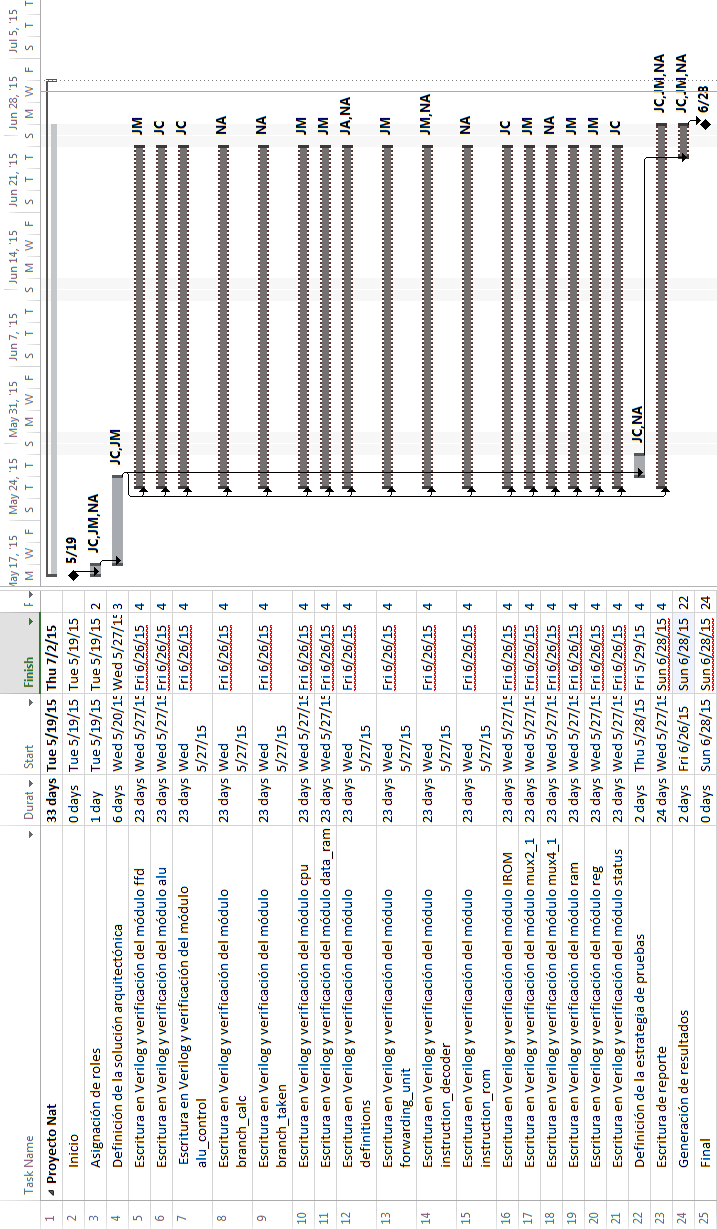
\includegraphics[scale=0.6]{imagenes/original.PNG}
\label{f:gannt_propuesto}
\end{figure}


\begin{figure}[hbtp]
\caption{Diagrama de Gannt Real}
\centering
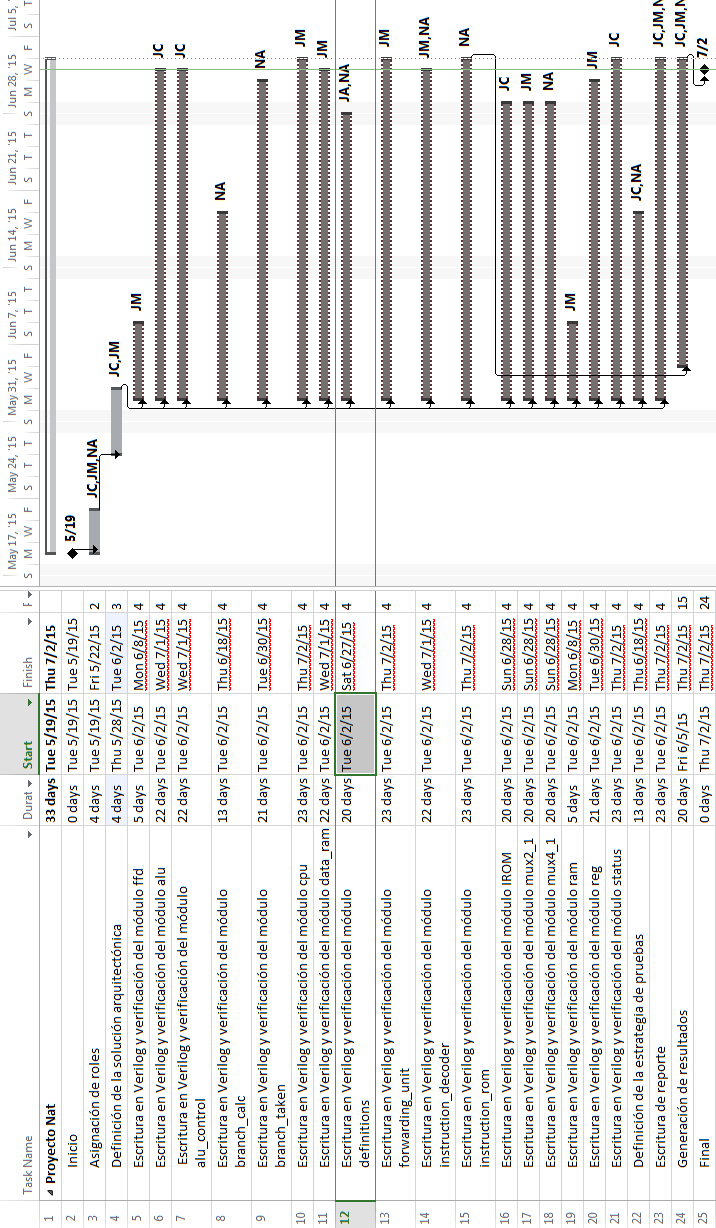
\includegraphics[scale=0.6]{imagenes/real.PNG}
\label{f:gannt_real}
\end{figure}

%%%%%%%%%%%%%%%%%%%%%%%%%%%%%

\newpage
%%%%%%%%%%%%%%
\section{Dise\~ no}
%%%%%%%%%%%%%%
\textit{Debe describir el dise\' ~o y su implementaci\' on. Se deben incluir diagramas de bloques o de estados, en caso de ser necesario. Deben explicar c\' omo funciona el dise\' ~o, y tener claro qu\' e elementos son clave de mencionar para que el lector pueda comprender c\' omo funciona el dise\' ~o. No incluya simulaciones en esta secci\' on, no incluya informaci\' on detallada del c\' odigo Verilog, la explicaci\' on debe ser de alto nivel. Debe brindarse una discusi\' on balanceada entre lo que usted implement\' o y porqu\' e se eligi\' o esa implementaci\' on. }

\subsection{Generalidades}
\subsection{Implementacion}
\subsection{Reto 1}
\subsection{Reto 2}

%%%%%%%%%%%%%%
\newpage
\section{Estrategia de pruebas}

\par Con el fin de comprobar el adecuado comportamiento de los multiplicadores implementados, se escribieron varios \textit{testbenches}, uno para cada multiplicador (dos, tres y cuatro entradas).
\\


\newpage
%%%%%%%%%%%%%%
\section{Evaluaci\' on}
%%%%%%%%%%%%%%

\par Para evaluar las pruebas planteadas en el apartado anterior, se ejecutaron los bancos de pruebas y se graficaron las se\~ nales resultantes (archivo signals.vcd), para analizar los resultados obtenidos.
\\
\par En los siguientes apartados se muestran los resultados obtenidos para cada uno de los multiplicadores.

\subsection{Banco de pruebas del decodificador de instrucciones}
El decodificador de instrucciones es el m\' odulo que se encarga de ajustar todas las se\~ nales de control del procesador de acuerdo a la instrucci\' on que se est\' a procesando en cada ciclo de reloj, de manera tal que debe ser capaz de obtener la decodificaci\' on de la instrucci\' on, las se\~ nales de control: \textit{write to a, write to b, mux pre alu a, mux pre alu b, read write, write back mux, jump, write mux y branch taken} de acuerdo al avance del contador de programa \textit{pc}.

Es de esta manera como se realiz\' o la simulaci\' on de las instrucciones que modifican las se\~ nales de control y se puede observar en la Figura \ref{fig:decoder} como efectivamente se tienen los resultados esperados de acuerdo con el dise\~ no del procesador.

\begin{figure}[hbtp]
\caption{Simulaci\' on del decodificador de instrucciones}
\centering
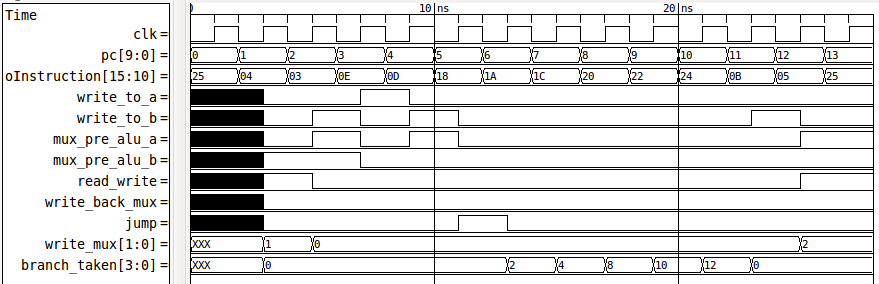
\includegraphics[scale=0.6]{../Codes/Verilog_Testbenches/scopes/Decoder_scope.png}
\label{fig:decoder}
\end{figure}


\subsection{Banco de pruebas de la ALU}
El m\' odulo ALU es el que se encarga de realizar el c\' alculo aritm\' etico de ciertas instrucciones que lo requieren y adem\' as obtener el valor de la se\~ nal de carry y la se\~ nal de cero. Tambien se encarga de realizar el c\' alculo de las direcciones de memoria para instrucciones que tienen que ver con el acceso o ingreso a la memoria principal.

De acuerdo con lo anterior y con la descripci\' on proporcionada en la secci\' on de dise\~ no se puede observar los resultados de la simulaci\' on efectuada en la Figura \ref{fig:alu} donde cabe destacar que el valor de los operandos \textit{in1, in2} y el resultado final \textit{out} se observa en formato decimal, mientras que las se\~ nales de \textit{carry} y \textit{zero} son bits.


\begin{figure}[hbtp]
\caption{Simulaci\' on de m\' odulo alu}
\centering
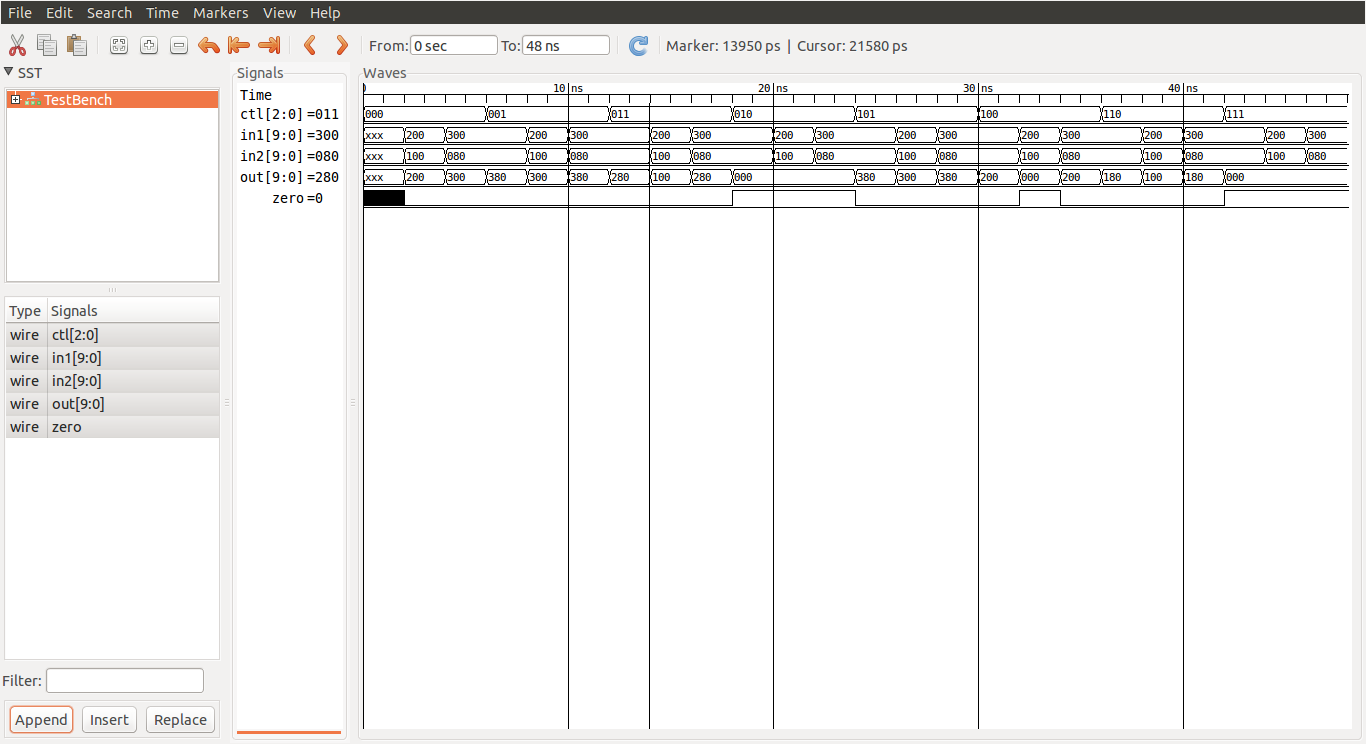
\includegraphics[scale=0.48]{../Codes/Verilog_Testbenches/scopes/ALU.png}
\label{fig:alu}
\end{figure}

\subsection{Banco de pruebas del controlador de ALU}
El m\' odulo controlador de la ALU es bastante importante en tanto que se encarga de obtener los bits de control que se encargan de decirle al m\' odulo ALU la tarea que debe desarrollar, por lo que en la evaluaci\' on de este m\' odulo se debe de tener como entrada todas las posibles instrucciones que se pueden ejecutar en el procesador y obtener a partir del c\' odigo de instrucci\' on, el c\' odigo de operando que debe implementar la ALU.

El resultado de la simulaci\' on se puede observar en la Figura \ref{fig:aluControl} donde se puede destacar que los c\' odigos de presentan en formato octal y adem\' as en orden de acuerdo con la descripci\' on presentada en la secci\' on de dise\~ no.

\begin{figure}[hbtp]
\caption{Simulaci\' on de m\' odulo controlador de alu}
\centering
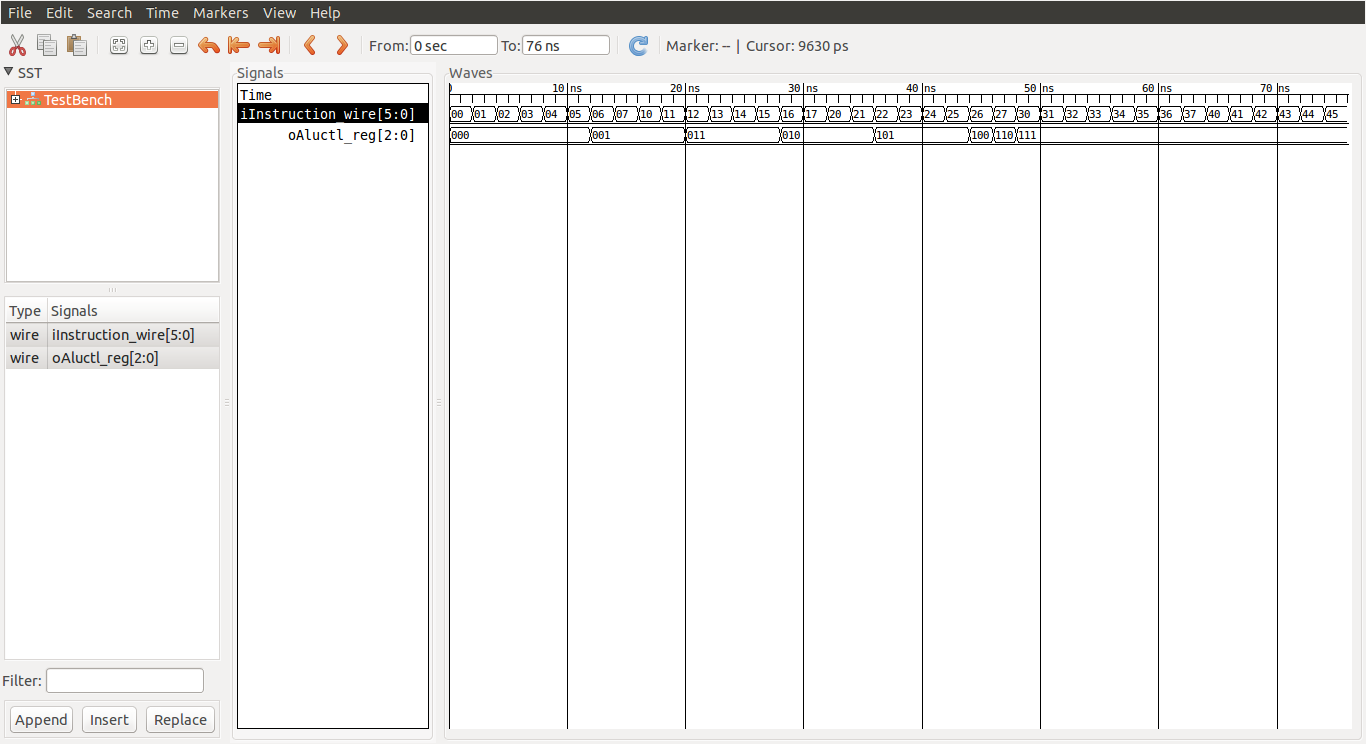
\includegraphics[scale=0.48]{../Codes/Verilog_Testbenches/scopes/ALU_Controller_scope.png}
\label{fig:aluControl}
\end{figure}


\subsection{Banco de pruebas del m\' odulo \textit{branch taken}}

\subsection{Banco de pruebas de las memorias}





\newpage
%%%%%%%%%%%%%%%%%%%
\section{Conclusiones}
%%%%%%%%%%%%%%%%%%%

\begin{itemize}

\item Una de las pricipales conclusiones que se obtienen al realizar el presente proyecto es comprender la importancia del uso de segmentaci\' on en los procesadores actuales en tanto que se puede obtener un desempe\~ no mucho mayor por el simple hecho de utilizar cada uno de los segmentos del procesador para tareas independientes y que de esta manera no se desperdicie tiempo de procesamiento, como si ocurre en los procesadores de ciclo simple.
\item Adem\' as de comprender el funcionamiento de un procesador segmentado mediante su implementaci\' on y dise\~ no en verilog, tambi\' en se logr\' o entender y comprender el efecto de los diferentes \textit{hazards} que se presentan aqu\' i y complican la labor de su desarrollo. De esta manera, el uso de unidades de \textit{forwarding} para procesadores segmentados es un deber que deber\' ia de tener siempre y cuando se busqu\' e mejorar el desempe\~ no del mismo.
\item Al igual que los puntos anteriores, el uso de m\' as de un registro en el procesador hace que el funcionamiento sea considerablemente m\' as complicado pues es necesario tomar en cuenta dependencia de instrucciones que normalmente no producen \textit{hazards}, tanto por el operando 1 como el operando 2.
\item Para lograr implementar una unidad l\' ogico arim\' etica, es necesario contar con un controlador de la misma, por lo cual una conclusi\' on que se obtuvo al respecto es que debe de existir un diagrama arquitect\' onico y un conjunto de instrucciones definidas mucho antes de realizar la implementaci\' on, y si se desean agregar nuevas instrucciones puede resultar en un cambio considerable del c\' odigo de programaci\' on.
\item Las instrucciones de ensamblador propuestas para el procesador son limitantes para diferentes aplicaciones y usos de las mismas, principalmente por no tener direccionamiento indirecto, interrupciones ni pila.
\item Por medio del uso de banderas se puede efectivamente determinar cuando un branch debe ser tomado.
\item Con respecto a la distribuci\' on de trabajo en grupo de logr\' o determinar que la distribuci\' on de las tareas debe ir de la mano con la modulaci\' on del esquema principal, lo cual simplifica mucho la ejecuci\' on del trabajo tanto aqu\' i como en cualquier otro proyecto pues permite a cada uno de los integrantes trabajar de manera independiente y tener un molde al cual apegarse para que el tiempo utilizado en la etapa de desarrollo sea lo menor posible.

\end{itemize}




%%%%%%%%%%%%%%
% Bibliograf\' ia
%%%%%%%%%%%%%%

\newpage

El formato recomendado para la bibliograf\' ia es el APA. El siguiente es un ejemplo:

\begin{thebibliography}{}
%\bibitem[Apuntes, 2008]{apuntes} \emph{http://www.apuntesdeelectronica.com/componentes/transistor-igbt.htm} consultado el 12/05/2013.
\bibitem[Morris y Ciletti, 2013]{Morris} M. Morris Mano y Michael D. Ciletti (2013). \emph{Dise\~ no Digital}. M\' exico:  Pearson Always Learning, 5th Edition.

\end{thebibliography}



%\newpage

%%%%%%%%%%%%%%
% Anexos
%%%%%%%%%%%%%%

%\appendix
%\section{Anexos}


%%%%% Transistor NTE123A y NTE159M
%%\subsection{Transistor 2N2222A}
%\includepdf[pages={1-3}]{./Anexos/2N2222A.pdf}





%%%%%%%%%%%%%%
\end{document}
%%%%%%%%%%%%%%
